% fig_improvement.tex
% Cumulative improvement bar chart: 87L baseline -> +87LN -> +TDCS
% Data: 12/21 (57%) -> 17/21 (81%) -> 21/21 (100%)
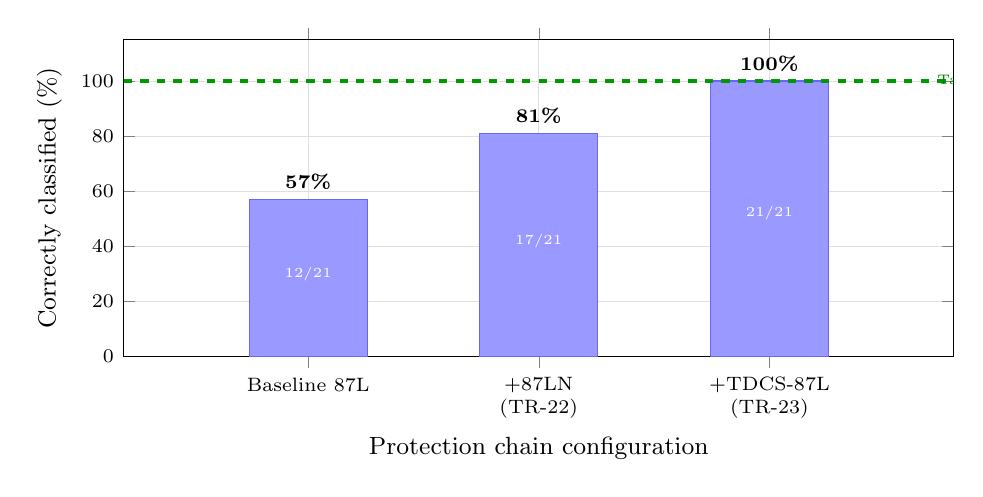
\begin{tikzpicture}
\begin{axis}[
  width=\columnwidth, height=5.6cm,
  ybar,
  bar width=1.5cm,
  xlabel={Protection chain configuration},
  ylabel={Correctly classified (\%)},
  xtick={1,2,3},
  xticklabels={Baseline 87L,{+87LN\\(TR-22)},{+TDCS-87L\\(TR-23)}},
  xticklabel style={font=\scriptsize,align=center,text width=2.5cm},
  xmin=0.2, xmax=3.8,
  ymin=0, ymax=115,
  ytick={0,20,40,60,80,100},
  yticklabel style={font=\scriptsize},
  grid=both,
  grid style={gray!25,line width=0.3pt},
  label style={font=\small},
  tick label style={font=\scriptsize}]

  % Bars
  \addplot[fill=blue!40,draw=blue!60] coordinates {
    (1, 57.1)
    (2, 81.0)
    (3, 100.0)
  };

  % Value labels
  \node[font=\scriptsize\bfseries,above] at (axis cs:1, 57.1) {57\%};
  \node[font=\scriptsize\bfseries,above] at (axis cs:2, 81.0) {81\%};
  \node[font=\scriptsize\bfseries,above] at (axis cs:3,100.0) {100\%};

  % Count labels inside bars
  \node[font=\tiny,white] at (axis cs:1, 30) {12/21};
  \node[font=\tiny,white] at (axis cs:2, 42) {17/21};
  \node[font=\tiny,white] at (axis cs:3, 52) {21/21};

  % Target line at 100%
  \draw[green!60!black,very thick,dashed]
    (axis cs:0.2,100) -- (axis cs:3.8,100)
    node[right,font=\tiny,green!50!black,xshift=-10pt]{Target};

\end{axis}
\end{tikzpicture}
